\deadline{2}{Designing the ER Model and converting it to a Relational Model}{February 3, 2023}

\section*{\Huge Entity-Relationship Model}
\vspace*{10pt}
Entity-Relationship (ER) Models are used to plan how different entities in a project interact with each other. \\
\newline
Our ER Model captures the nature of the relationships and entities planned to be used in the project.
The ER Model is designed in accordance with the assumptions and constraints as mentioned in the document above.
Hence, we plan to build our system on the basis of the following Entity-Relationship Model:
\vspace*{10pt}
\begin{center}
    \hspace*{-37pt}
    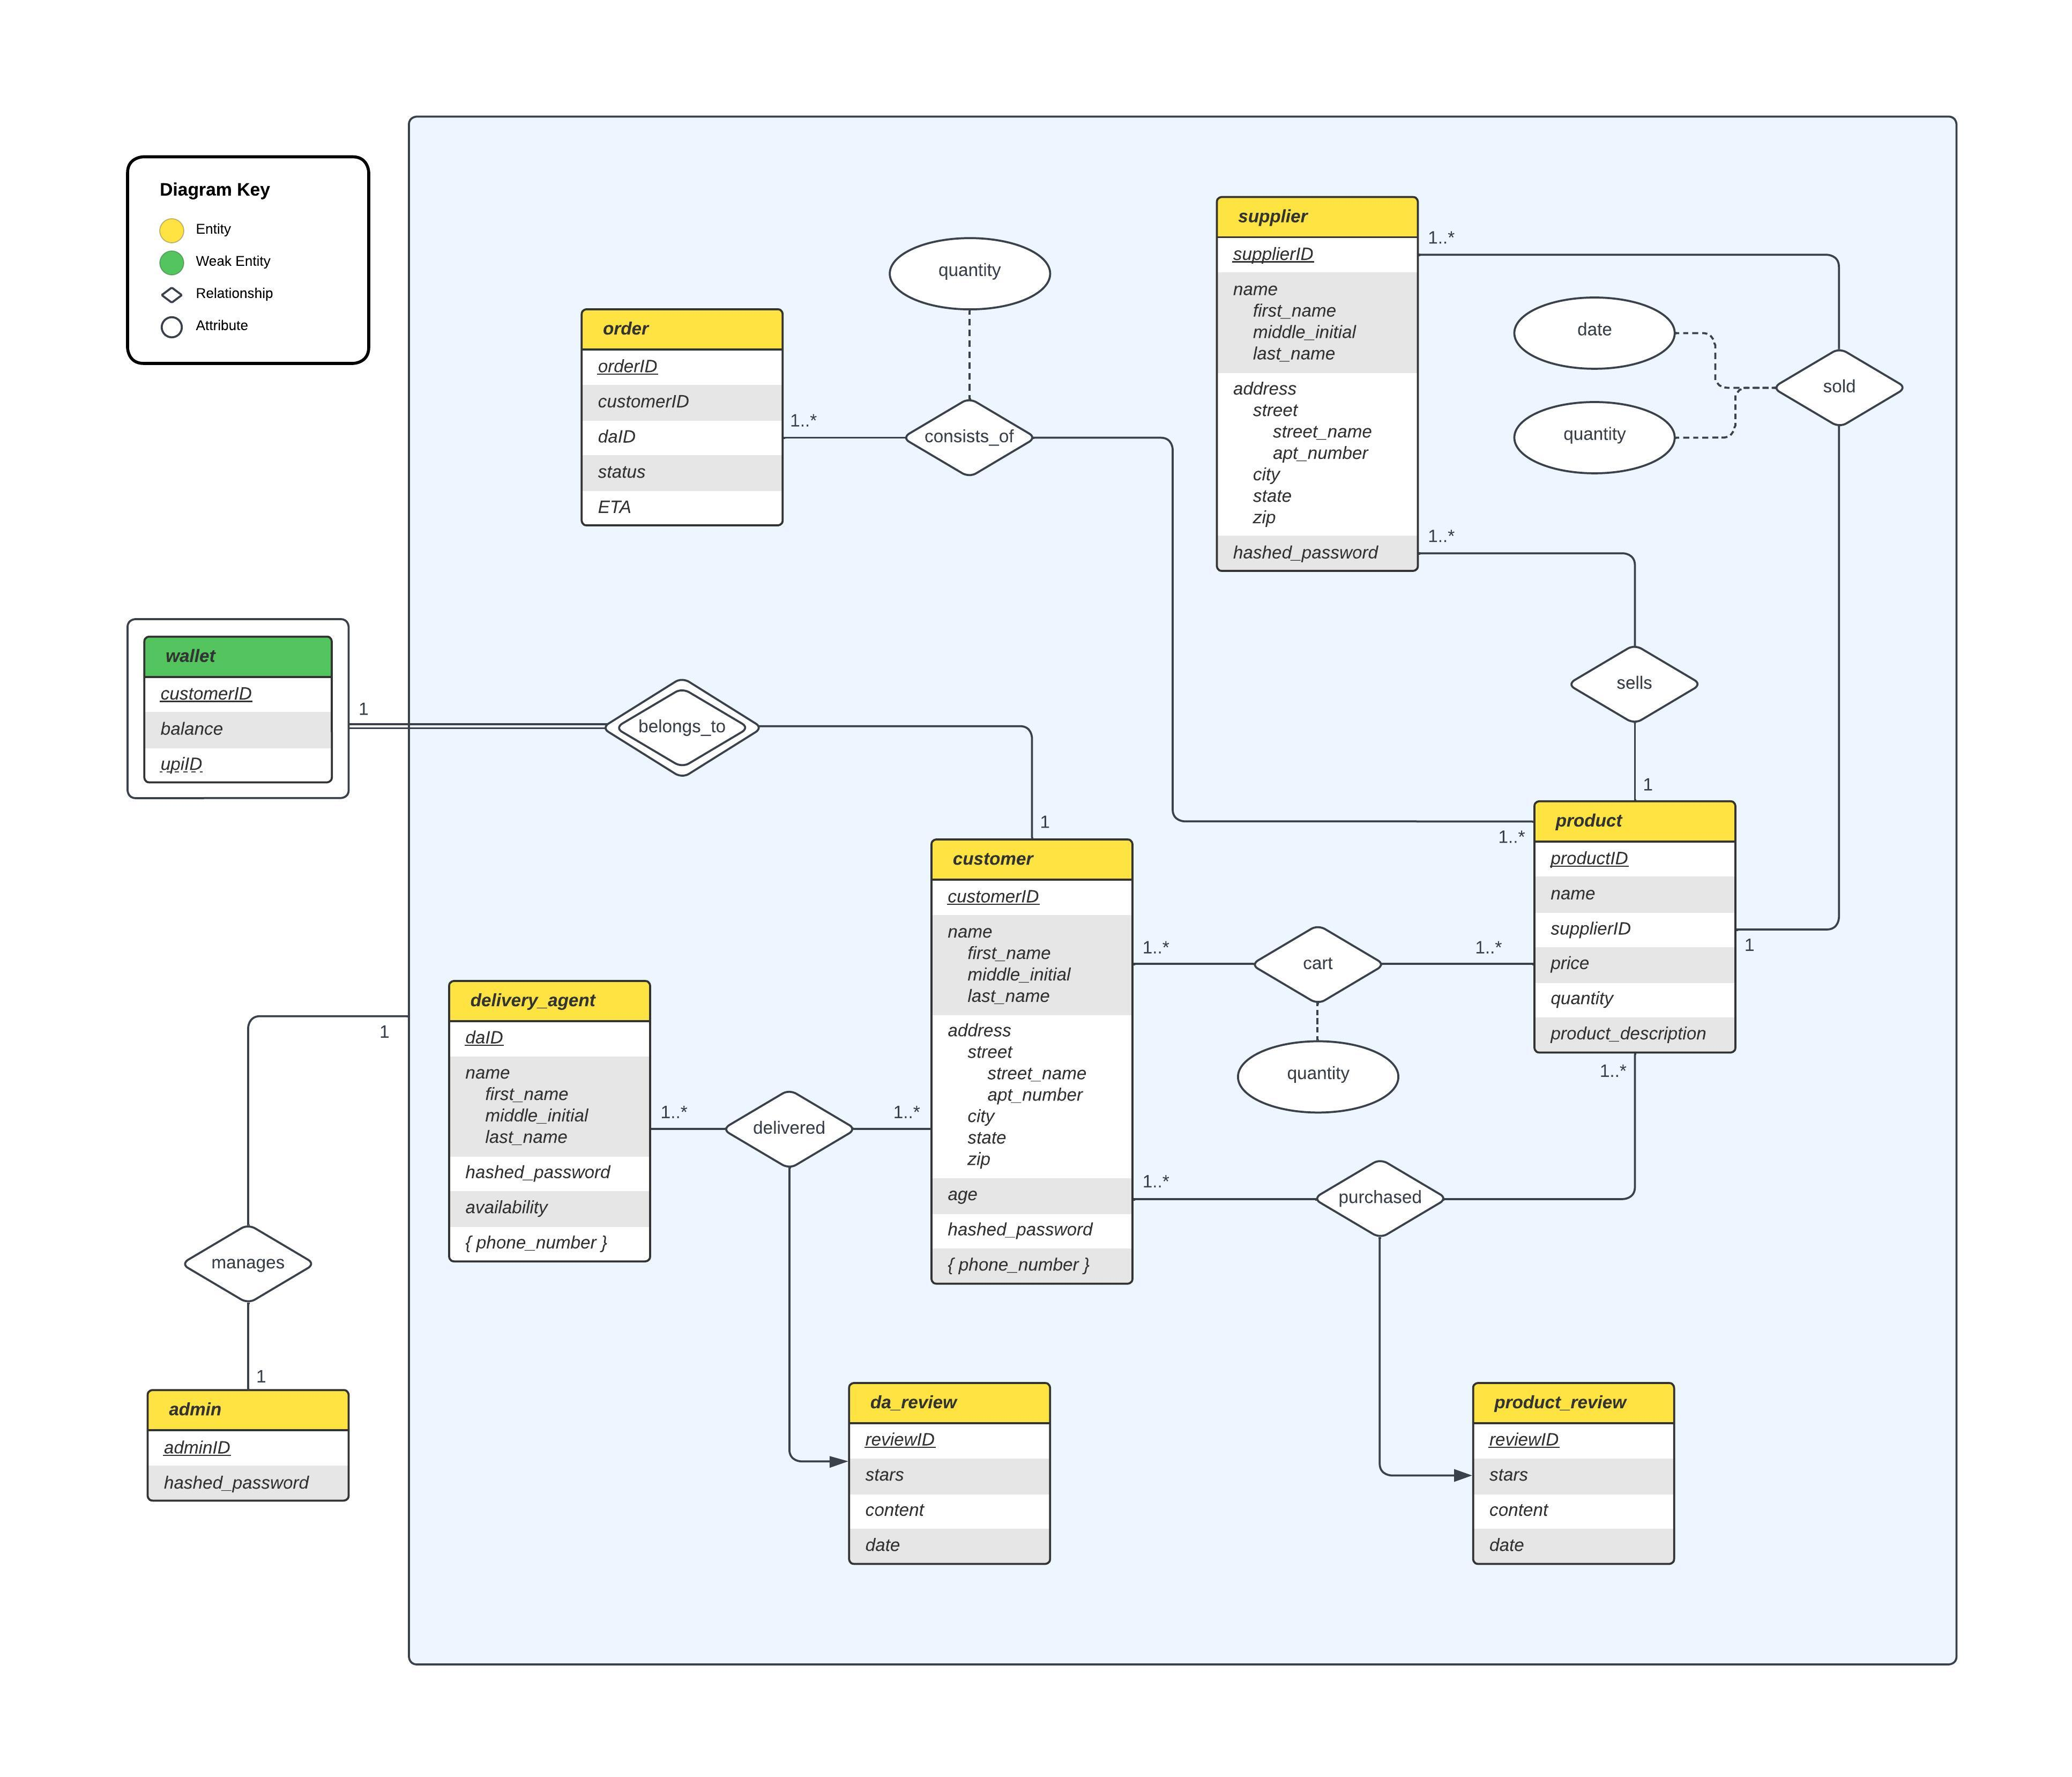
\includegraphics[scale=0.6]{ER-Model}
\end{center}

\subsection*{Ternary Relationships}
The following ternary relationships have been identified:
\begin{enumerate}
    \item \textbf{Customer - Product - Product Review:}
    A customer can review multiple products, and a product can be reviewed by multiple customers.
    A customer can give at most one review per product.
    This ternary relationship will be decomposed into the following binary relationships at the time of implentation:
    \begin{enumerate}
        \item \textbf{Customer - Product:}
        (Many-to-Many) To keep track of which customers have purchased which products.
        \item \textbf{Product - Product Review:}
        (One-to-Many) To keep track of all reviews given to a product.
        \item \textbf{Customer - Product Review:}
        (One-to-Many) To keep track of all reviews given by a customer.
        This relationship may not be needed and may be removed in the future.
    \end{enumerate}
    \item \textbf{Delivery Agent - Customer - Delivery Agent Review:}
    A customer can review multiple delivery agents, and a delivery agent can be reviewed by multiple customers.
    A customer can give at most one review per delivery agent.
    This ternary relationship will be decomposed into the following binary relationships at the time of implentation:
    \begin{enumerate}
        \item \textbf{Customer - Delivery Agent:}
        (Many-to-Many) To keep track of which customers have received orders from which delivery agents.
        \item \textbf{Delivery Agent - Delivery Agent Review:}
        (One-to-Many) To keep track of all reviews given to a delivery agent.
        \item \textbf{Customer - Delivery Agent Review:}
        (One-to-Many) To keep track of all reviews given by a customer.
        This relationship may not be needed and may be removed in the future.
    \end{enumerate}
\end{enumerate}

\section*{\Huge Relational Model}
\vspace*{10pt}
Relationship Models are used to represent how data will be stored in the database, along with the attributes of each entity and relationship.
The Relational Model is designed in accordance with the assumptions and constraints as mentioned in the document above. \\
\newline
\textbf{Note:} The arrows represent that a field is \textit{derived} from another.
For example, \texttt{productID} in \texttt{description} will contain values of \texttt{productID} from table \texttt{product}.
\pagebreak
\vspace*{35pt}
\begin{center}
    \hspace*{-40pt}
    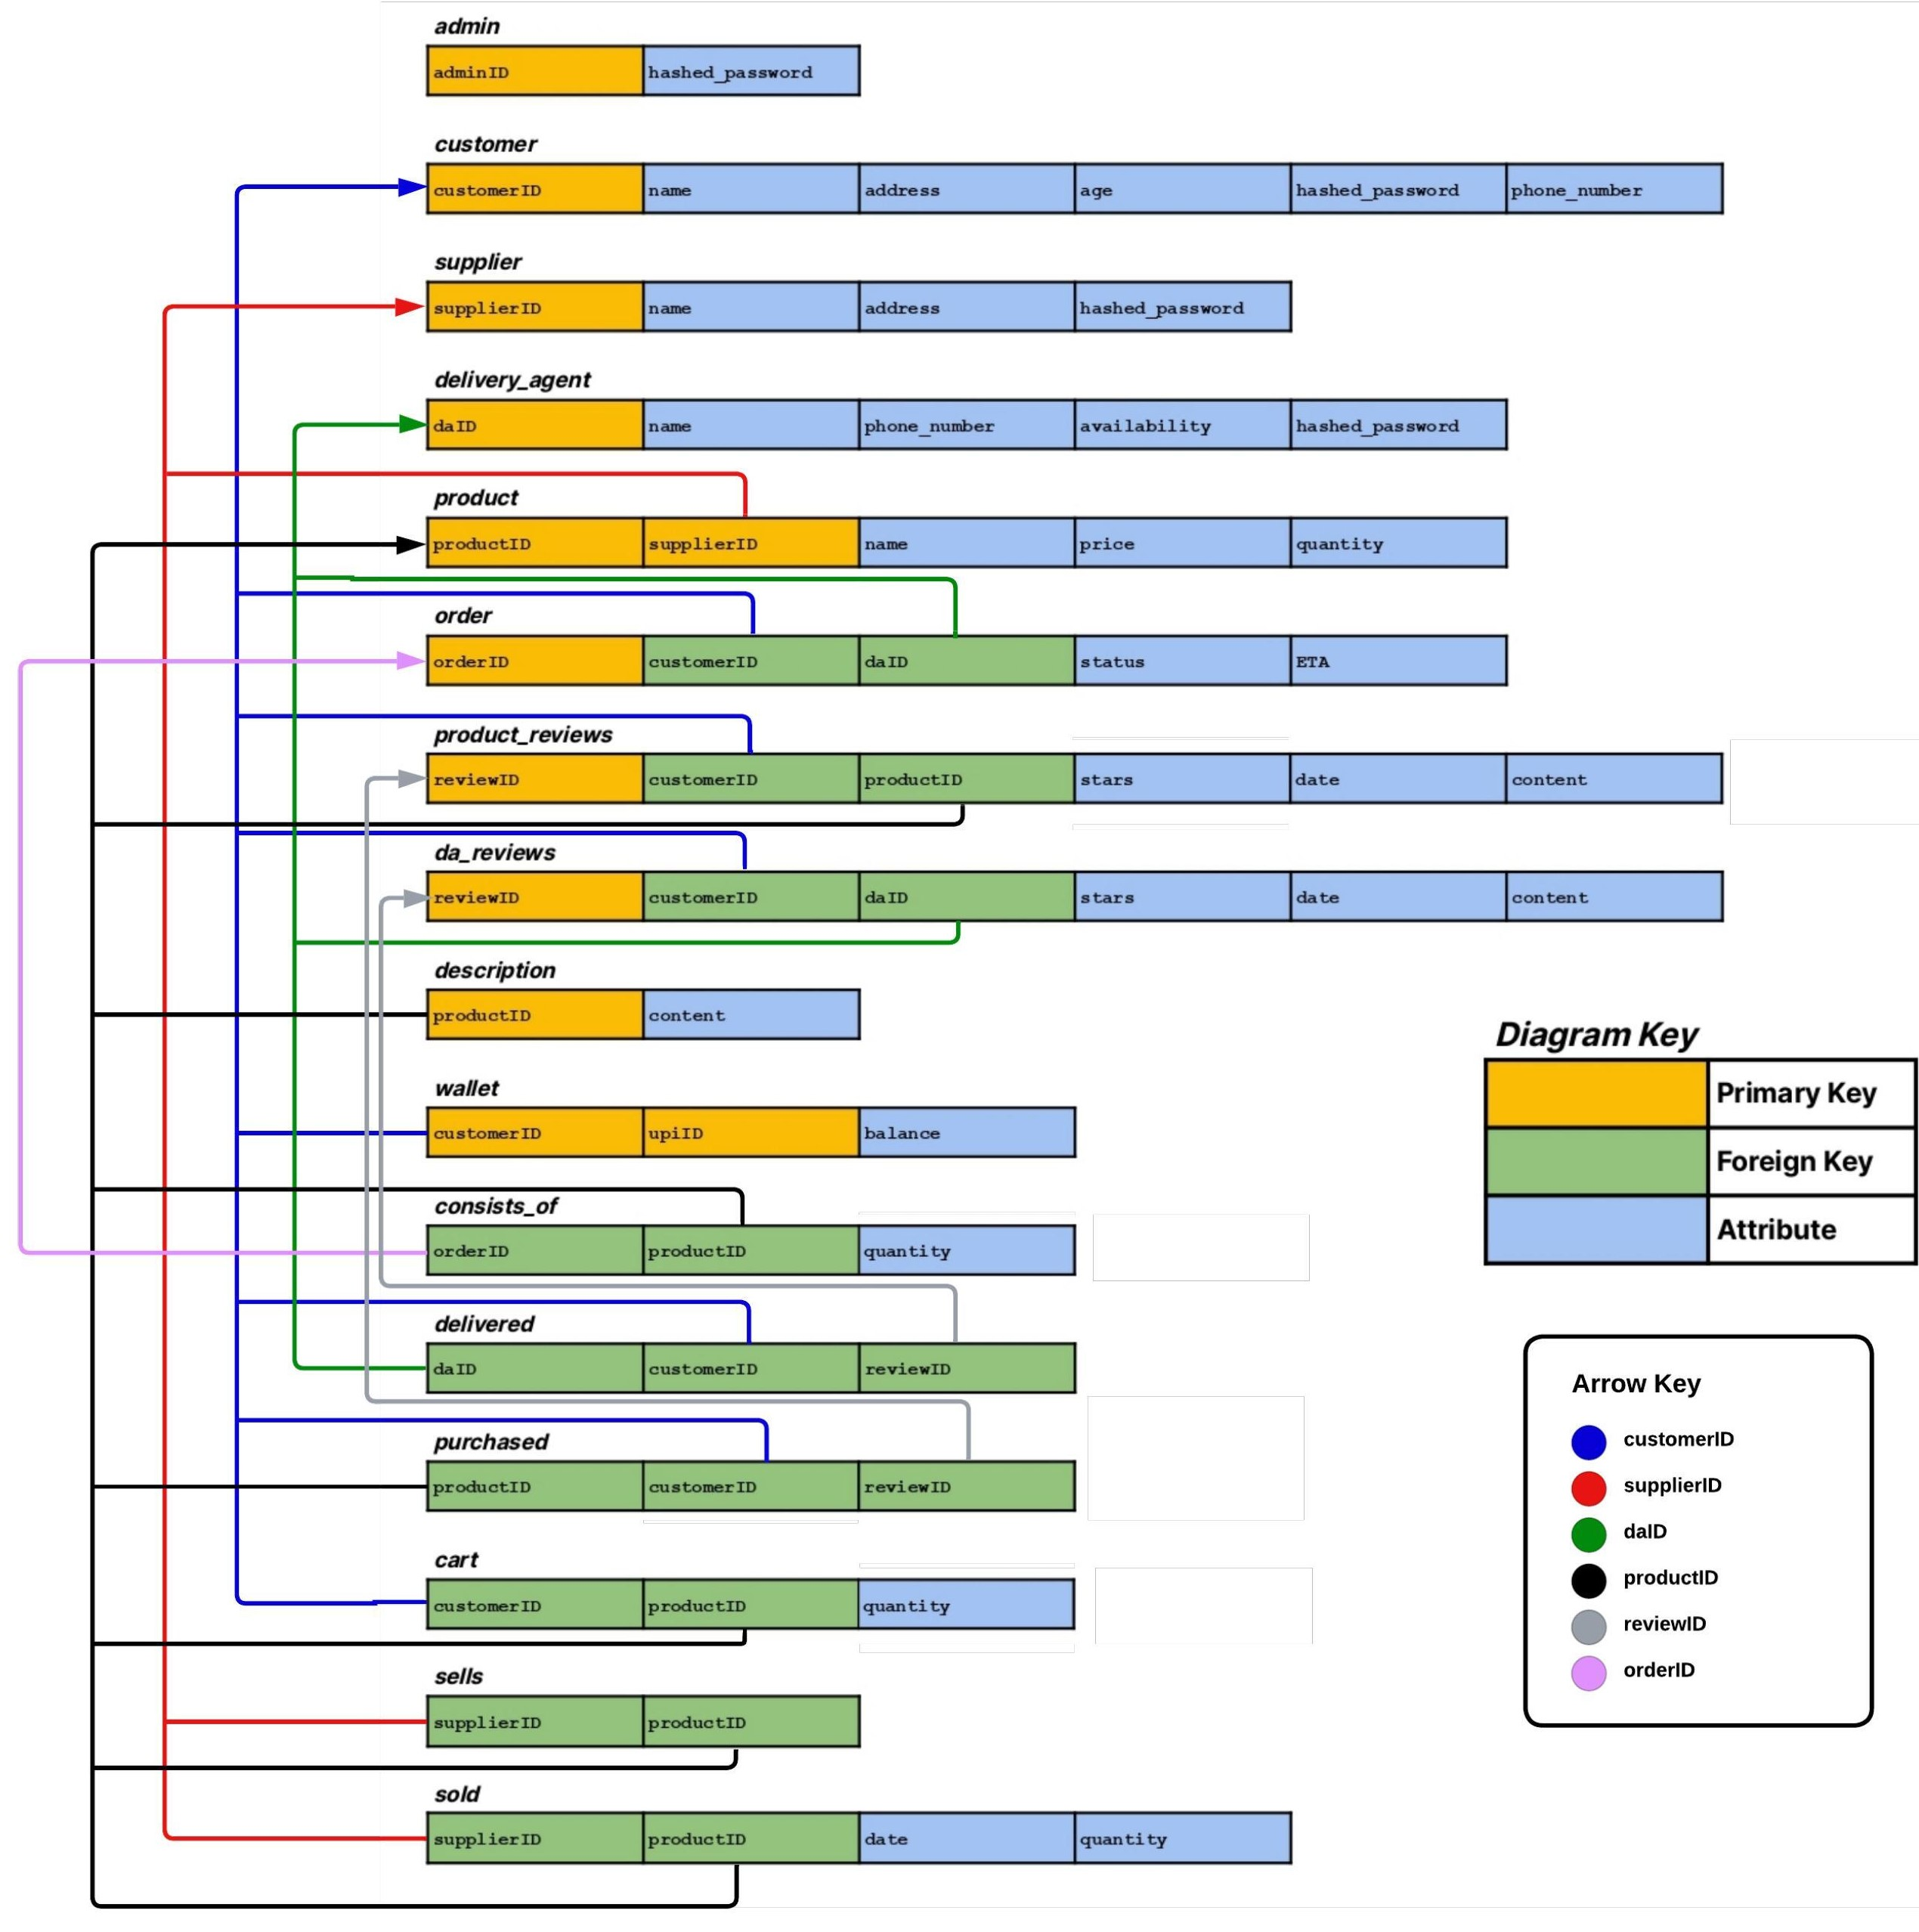
\includegraphics[scale=0.8]{Relational-Model}
\end{center}

\pagebreak